\documentclass{report}
\usepackage{polyglossia}
\usepackage{graphicx}
\usepackage{fixlatvian}
\usepackage{verbatim}
\usepackage{circuitikz}
\usepackage{pgfplots}
\title{vienkāršu elektrisku shēmu modelēšana}
\author{Rinalds Štauers }

\begin{document}
\maketitle
%=================================
\chapter{Teorētiskā daļa}
Te es rakstīšu teorētisko daļu
%=================================
\section{ķēdes aprēķins}
Aprēķinam spriegumus uz rezistoriem. Sprieguma avota V1 sprieguma vērtību izvēlas daļskaitli, kas būtu studenta apliecības pēdējie trīs cipari dalīti ar skaitli 10. R1 ir apliecības pēdējo trīs ciparu otrais cipars, kuram pieskaita 1. R2 ir apliecības numura pēdējais cipars, kuram arī piesakitla 1. Piemēram : 161RIC028 V1 = 28/10 = 2,8, R1 = 2+1=3 un R2 = 8+1=9.Ur1 = V1 * R1 un Ur2 = V1 * R2.
%=======================================
\begin{figure}
\begin{center}
\begin{circuitikz}[american voltages]
\draw
(0,4) to [V, l_=$Us$] (0,0)
to [short, *-] (6,0)
to (6,2)
to [R, l_=$R$] (6,4)
to [short, ] (5,4)
to (3,4) to [open, ] (0,4)
to [short, ] (1,4)
to [R, l=$R$] (3,4)
to (4,4)
;
\end{circuitikz}
\end{center}
\caption{Elektriskā shēma}
\end{figure}
\newpage


\begin{table}
\begin{tabular}{|c|c|}
\hline
   R1  & 3 \\
   \hline
    R2 & 9 \\
    \hline
    V1 & 2,8 \\
    \hline
    Ur2 & 25,2 \\
    \hline
    Ur1 & 8,4 \\
    \hline
\end{tabular}
\begin{centering}
\caption{Sprieguma un pretestību tabula}
\end{centering}
\end{table}
\newpage
\begin{figure}
    \centering
    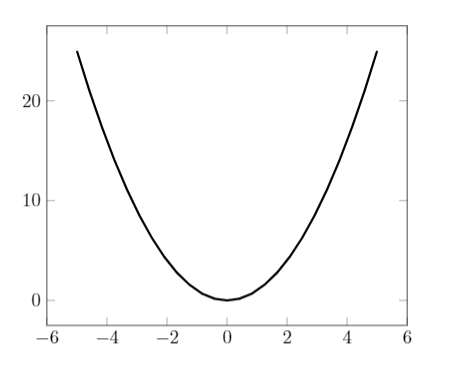
\includegraphics[width=10cm]{grafiks.png}
    \caption{sprieguma grafiks}
\end{figure}


\chapter{Praktiskā daļa}
\section{Darbs ar GEDA programmām}
\subsection{darbs ar gscheme}

\begin{figure}[!h]
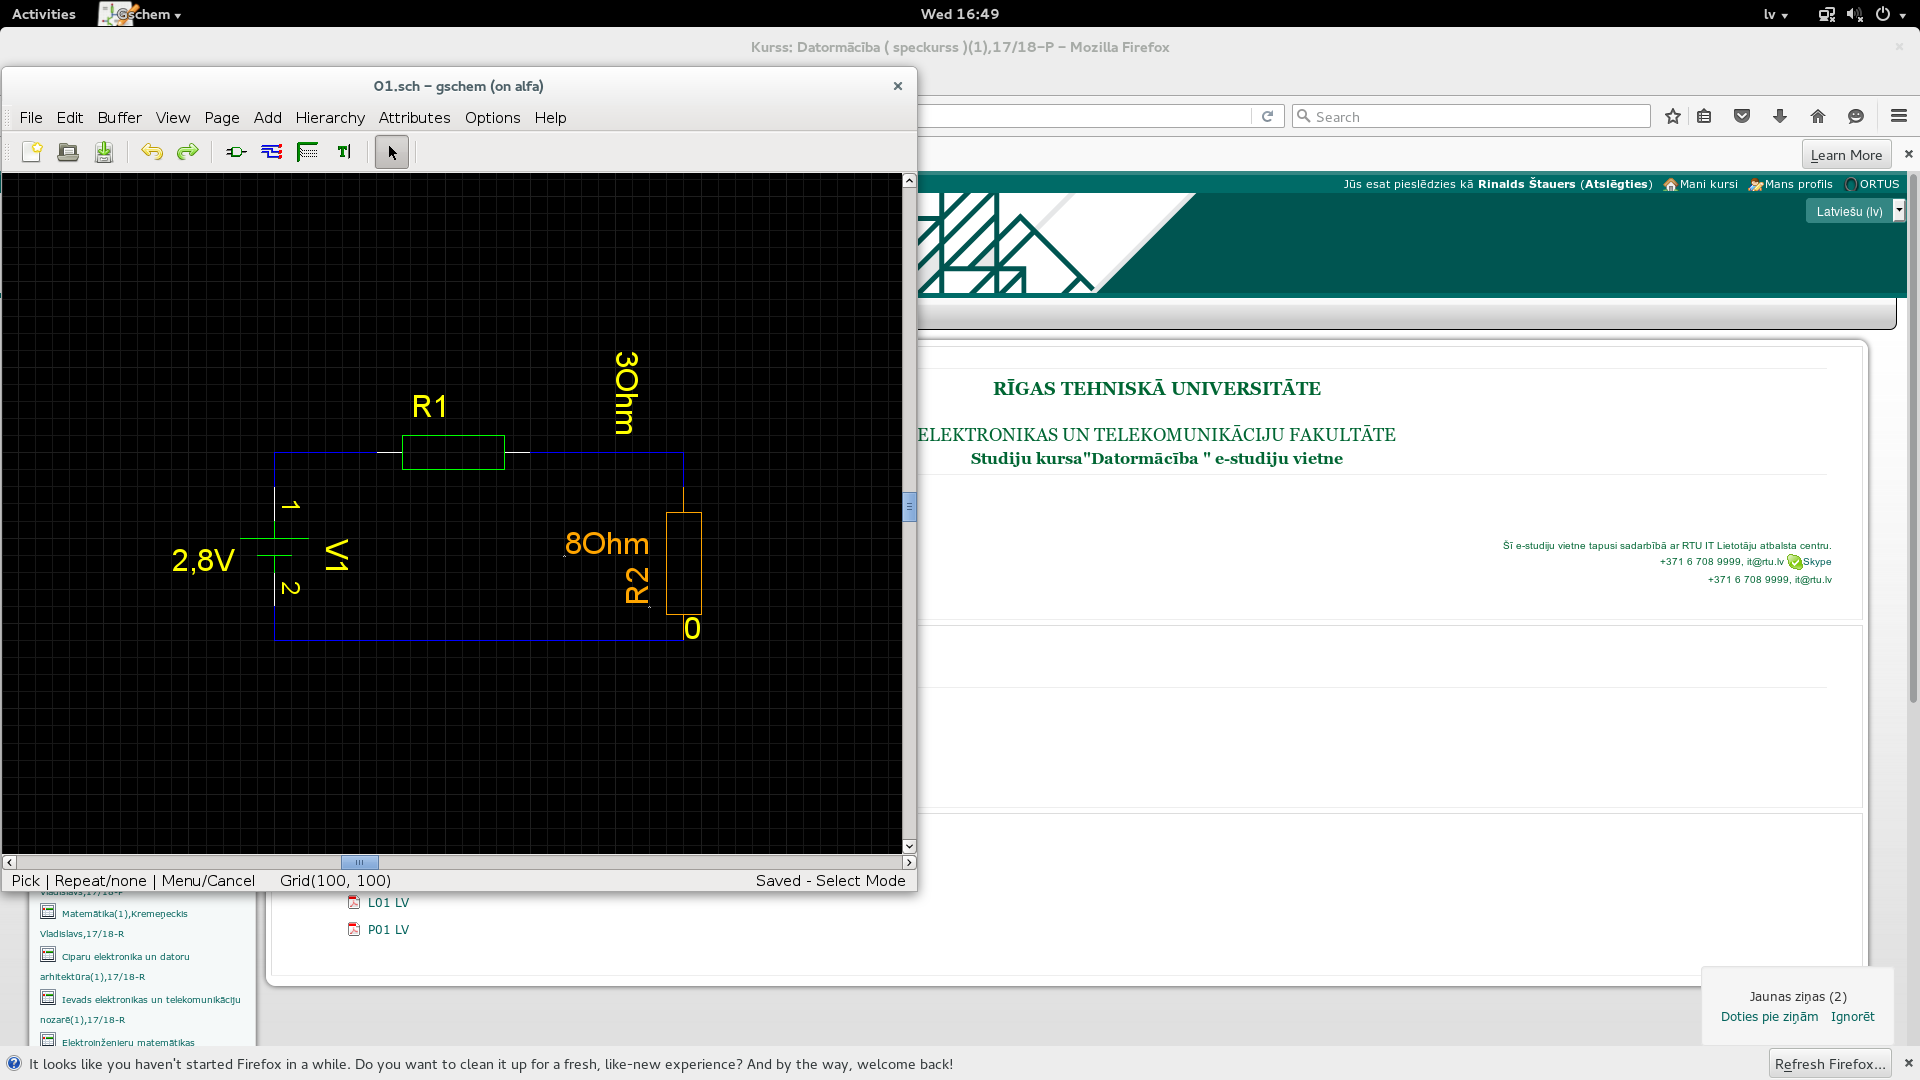
\includegraphics[width=\textwidth]{shema.png}
\caption{Elektriskā shēma}

\end{figure}
\newpage
\subsection{darbs ar gentlist}
\verbatiminput{01.net}

\subsection{darbs ar ngspice}
\begin{figure}[!h]
\includegraphics[widths=10cm, height=10cm]{grafiks.ps}
\caption{NGspice izveidotais grafiks}


\end{figure}


\begin{figure}

\section{Darbs QUCS programmām}
\rotatebox{-90}{\includegraphics[width=15cm, height=30cm]{qucs.ps}}
\caption{QUCS izveidotā ķēde}
\end{figure}

\begin{figure}
\subsection{Sweep grafiki}
\rotatebox{-90}{\includegraphics[width=15cm]{g1.ps}}
\caption{Sweep izveidotais grafiks}
\end{figure}


\newpage
\begin{figure}
\subsection{Sweep Tabula}
\rotatebox{-90}{
\includegraphics[width=25cm]{tabula.ps}}
\caption{Sweep izveidotā tabula}
\end{figure}




\newpage
\subsection{Secinājumi}
1) Parameter sweep programma palīdz ātri un viegli saslēgt ķēdi ar sev nepieciešamajiem elementiem.
\vspace{5mm}
\newline
2) Geda programma palīdz viegli iegūt grafikus par izveidotajām ķēdēm.
\vspace{5mm}
\newline
3) Ar sharelatex palīzību ir viegli sataisīt pārskatāmu atskaiti par veikto darbus.
\vspace{5mm}
\newline
4) Ļoti viegli uztaisīt attēlu sarakstu, atsaucoties uz attēliem, ka arī grafikiem no darba.


\listoffigures

\end{document}
